Klasifikuojant daugiamačius duomenis susiduriame su taip vadinamu dimensiškumo
prakeiksmu (angl. curse of dimentionality). Pavyzdžiui, kai dimensijų skaičius įkopia į
trečią ar ketvirtą eilę naudoti paprastus klasifikavimo algoritmus tampa
nebeefektyvu nei laiko, nei klasifikavimo našumo atžvilgiais. Vienas iš būdų
kovoti su dimensiškumo prakeiksmu
yra naudoti vienokius ar kitokius dimensijų skaičiaus mažinimo metodus. Šiame
skyriuje nagrinėsiu bazinius dimensijų atsirinkimo metodus, keletos 
kriterijų suliejimą metodą (angl.
feature selection based on multicriterion fusion)\cite{yang2011robust}, bei
stabilių dimensijų grupių išskyrimo metodą\cite{Loscalzo:2009:CGS:1557019.1557084}.

\subsection{Baziniai dimensijų atrinkimo metodai}

Yra pasiūlyta daugybė dimensijų atrinkimo metodų. Šiame skyriuje aptarsiu
keletą taip vadinamų bazinių\footnote{Aptarsiu tik bazinius todėl, kad jie yra 
svarbiausi, nes jų tarpusavio rezultatai yra nekoreliuojantys, o nekoreliuojančius
rezultatus galima panaudot juos apjungiant, taip gauname sinergijos efektą.}
dimensijų atrinkimo metodų: 
\begin{enumerate}
 \item Fisher'io įvertis (angl. Fisher ratio)\cite{Pavlidis:2001:GFC:369133.369228};
 \item Atpalaidavimo (ang. relief) metodas\cite{DBLP:journals/ml/Robnik-SikonjaK03};
 \item Asimetrinis priklausomybės koeficientas\cite{Shannon:2001:MTC:584091.584093} (ADC) (angl.
 Asymmetric Dependency Coefficient);
 \item Absoliučių svorių SVM\cite{vapnik2000nature} (AW-SVM) (angl. Absolute Weight SVM)
 \item Rekursyvus dimensijų eliminavimas pagal SVM\cite{Guyon:2002:GSC:599613.599671} (SVM-RFE) (angl. Recursive
 Feature Elimination by SVM)
\end{enumerate}

\subsubsection{Fisher'io įvertis}

Fisher'io įvertis vertina individualias dimensijas pagal jų klasių atskiriamąją 
galią. Dimensijos įvertis yra sudarytas iš tarpklasinio skirtumo santykio su 
vidiniu klasės pasiskirstymu:
\begin{equation}
 FR(j) = \frac{(\mu_{j1} - \mu_{j2})^2}{\sigma_{j1}^2 + \sigma_{j2}^2},
\end{equation}
kur, $j$ - yra dimensijos indeksas, $\mu_{jc}$ - dimensijos $j$ reikšmių vidurkis
klasėje $c$, $\sigma_{jc}^2$ - dimensijos $j$ reikšmių standartinis nuokrypis
klasėje $c$, kur $c={1,2}$. Kuo didesnis yra Fisher'io įvertis, tuo geriau ta
dimensija atskiria klases.

\subsubsection{Atpalaidavimo metodas}

Atpalaidavimo metodas iteratyviai skaičiuoja dimensijų ,,susietumą``. Pradžioje
,,susietumas`` visoms dimensijoms yra lygus nuliui. Kiekvienoje
iteracijoje atsitiktinai\footnote{Pastebėtina, kad metodas 
turi atsitiktinį elementą, todėl klasifikavimo ir  dimensijų atrinkimo stabilumo
rezultatai dažniausiai šiek tiek varijuoja nekeičiant konfigūracijos.} 
pasirenkamas objektas iš duomenų bazės, surandami
artimiausi kaimynai iš tos pačios ir kitos klasės, ir atnaujinamos visų 
dimensijų ,,susietumo`` reikšmės. Dimensijos įvertis yra vidurkis visų objektų
atstumų iki artimiausių kaimynų iš tos pačios ir kitos kasės:
\begin{equation}
 W(j)=W(j) - \frac{diff(j, x, x_H)}{n} + \frac{diff(i, x, x_M)}{n},
\end{equation}
kur $W(j)$ - $j$-osios dimensijos ,,susietumo`` įvertis, $n$ - objektų aibės 
dydis,$x$ - atsitiktinai pasirinktas objektas, $x_H$ - artimiausias
kaimynas iš tos pačios klasės (angl. nearest-Hit), $x_M$ - artimiausias kaimynas
iš kitos klasės, $diff(j, x, x')$ - $j$-osios dimensijos reikšmių skirtumas
tarp laisvai pasirinkto objekto $x$ ir atitinkamo kaimyno, kur skirtumą į
intervalą $[0, 1]$ normalizuojanti funkcija yra:
\begin{equation}
 diff(j, x, x')=\frac{|x_j- x_j'|}{x_{j max} - x_{i min}},
\end{equation}
kur $x_{j max}$ ir $x_{j min}$ yra maximali ir minimali $j$-osios dimensijos
reikšmės. ,,Susietumo`` reikšmių atnaujinimas yra vykdomas $n$ kartų ir kuo
didesnė galutinė reikšmė, tuo svarbesnė dimensija. Pastebėtina, kad šis algoritmas
veikia tik su dviejomis klasėmis, nors yra ir išplėtimų.

\subsubsection{Asimetrinis priklausomybės koeficientas}

Asimetrinis priklausomybės koeficientas yra dimensijų reitingavimo motodas,
kuris matuoja klasės $Y$ etiketės (angl. label) tikimybinę priklausomybę $j$-ąjai
dimensijąi, naudodamas informacijos prieaugį (angl. information gain):
\begin{equation}
 ADC(Y, j) = \frac{MI(Y, X_j)}{H(Y)},
\end{equation}
kur $H(Y)$ - klasės $Y$ entropija, o $MI(Y, X_j)$ - yra bendrumo informacija
(angl. mutual information) tarp klasės etiketės $Y$ ir $j$-osios dimensijos
\begin{equation}
 H(Y)=-\sum_y{p(Y=y)log{p(Y=y)}}, 
\end{equation}
\begin{equation}
 H(X_j)=-\sum_x{p(X_j=x) log{p(X_j=x)}},
\end{equation}
\begin{equation}
 MI(Y, X_j) = H(Y) + H(X_j) - H(Y, X_j),
\end{equation}
\begin{equation}
 H(Y, X_j) = -\sum_{y,x_j}{p(y, x_j)log{p(y, x_j)}},
\end{equation}

Kuo didesni ADC įverčiai, tuo dimensija yra svarbesnė, nes turi daugiau
informacijos apie duomenų klases.

\subsubsection{Absoliučių svorių SVM}

Atraminių vektorių metodas (SVM) yra vienas populiariausių klasifikavimo algortimų,
nes jis gerai susidoroja su daugiamačiais duomenimis. Yra keletas bazinių 
SVM variantų, bet šiame darbe naudosime tiesinį SVM, nes jis demonstruoja
gerus rezultatus dirbant su genų ekspresijos duomenimis. Tiesinis SVM yra
hiperplokštuma apibrėžta kaip:
\begin{equation}
 \sum_{j=1}^{p}{w_jx_j + b_0 = 0},
\end{equation}
kur $p$ - dimensijų kiekis, $w_j$ - j-osios dimensijos svoris, $x_j$ - j-osios
dimensijos kintamasis, $b_0$ - konstanta. Dimensijos absoliutus\footnote{Svorį
reikia imti absoliutaus dydžio, nes neigiamas svoris implikuoja priklausomybę 
vienai klasei, o teigiamas kitai klasei.} svoris $w_j$ gali būti panaudotas
dimensijų reitingavimui. Pastebėtina, kad svorių nustatymas yra atliekamas tik 
vieną kartą\footnote{SVM-RFE - metodas svorius nustato daug kartų.}.

\subsubsection{Rekursyvus dimensijų eliminavimas pagal SVM}

Rekursyvus dimensijų eliminavimas pagal SVM yra vienas populiariausių dimensijų
atrinkimo algoritmų. Todėl, jis yra naudojamas, kaip atskaitos taškas (angl. threshold)
vertinant
kitus dimensijų atrankos metodus. Iš esmės šis metodas yra daugkartinis 
absoliučių svorių SVM metodo taikymas nuolat išmetinėjant dimensijas su 
mažiausiais svoriais. Rekursyvus dimensijų eliminavimas mums padeda surasti 
tinkamą dimensijų poaibį, kas nevisada pavyksta su dimensijų reitingavimo 
metodais. Bendroji rekursyvaus dimensijų eliminavimo procedūra:
\begin{algorithm}
\caption{Rekursyvus dimensijų eliminavimas}
\label{RFE}
 \begin{enumerate}
 \item Turime pilną dimensijų rinkinį $F_0$, nustatome $i=0$.
 \item Įvertiname kiekvienos dimensijos kokybę dimensijų aibėje $F_i$.
 \item Išmetame mažiausiai svarbią dimensiją iš $F_I$ tam, kad gautume
 dimensijų rinkinį $F_{i+1}$.
 \item Nustatome $i=i+1$ ir grįžtame į antrąjį žingsnį kol nėra patenkinta 
 algoritmo pabaigos sąlyga.
\end{enumerate}
\end{algorithm}
Jei trečiajame algoritmo žingsnyje yra pašalinama tik viena dimensija, tai gauname dar
ir dimensijų reitingavimą, o jei pašalinamos kelios dimensijos ar jų dalis
(pvz. 50\%) tai reitingavimo negauname. Pastebėtina, kad rekursyvus dimensijų
eliminavimas gali labai padidinti algoritmo sudėtingumą skaičiavimo resursų
atžvilgiu. Algoritmo pabaigos sąlyga gali būti koks nors konkretus dimensijų
skaičius arba tiesiog dimensijų aibę mažinti tol, kol dimensijų visai nebeliks.

\subsection{Multikriterinis dimensijų atrinkimas}

Multikriterinio dimensijų atrinkimo metodų esmė yra panaudoti
kelis dimensijų atrinkimo metodus suliejant jų
rezultatus į vieną bendrą rezultatą. Kodėl naudinga sulieti keletą dimensijų
atrinkimo metodų rezultatų? Sulieti keletą dimensijų atrinkimo metodų rezultatų
naudinga, nes
pavieniai dimensijų atrinkimo metodai be to, kad turi savitų privalumų, visada
turi ir savo silnybių, pavyzdžiui, jautrumas išimtims (angl. outliers), negali
rasti dimensijų tarpusavio priklausomybių, etc. Yra skiriamos trys priežastys,
kodėl keletas kombinuotų silpnų ir nestabilių dimensijų atrinkimo metodų
gali duoti geresnius rezultatus\cite{dietterich2000ensemble}:
\begin{enumerate}
 \item Keletas skirtingų, bet vienodai optimalių hipotezių gali būti teisingos,
 ir kriterijų kombinavimas sumažiną tikimybę, kad bus pasirinkta neteisinga 
 hipotezė;
 \item Atskiri kriterijai gali dirbti skirtinguose lokaliuose optimumuose, tuo
 tarpu kombinavimas gali geriau reprezentuoti tikrąją duomenų funkciją;
 \item Tikroji duomenų funkcija negali būti reprezentuojama jokia hipoteze
 paskiro algoritmo hipotezių erdvėje ir agreguojant pavienių metodų rezultatus
 galima praplėsti hipotezių erdvę.
\end{enumerate}
Suliejant keletą skirtingų metodų
suliejamos gerosios pavienių dimensijų atrinkimo metodų savybės, taip
kompensuojant algoritmų silpnybes.

Galima pavienių dimensijų atrankos rezultatus sulieti pagal šias suliejimo
strategijas:
\begin{enumerate}
  \item Svoriais grįstas multikriterinis suliejimas;
  \item Reitingais (angl. rank) grįstas multikriterinis suliejimas;
  \item Svoriais ir reitingais grįstas multikriterinis suliejimas.
\end{enumerate}

\subsubsection{Svoriais grįstas multikriterinis suliejimas}

Svoriais grįsto multikriterinio dimensijų atrinkimo suliejimo pagal svorius algoritmo
pirmajame žingsnyje kiekvienas bazinis metodas priskiria duomenų rinkinio
dimensijoms svorius, tada tie svoriai yra kombinuojami į vieną sutarties
(angl. consensus) svorių vektorių, kurio pagrindu yra gaunami dimensijų 
reitingai. Algoritmas yra pavaizduotas ~\ref{fig:figure4} pav.
\begin{figure}
 \centering
 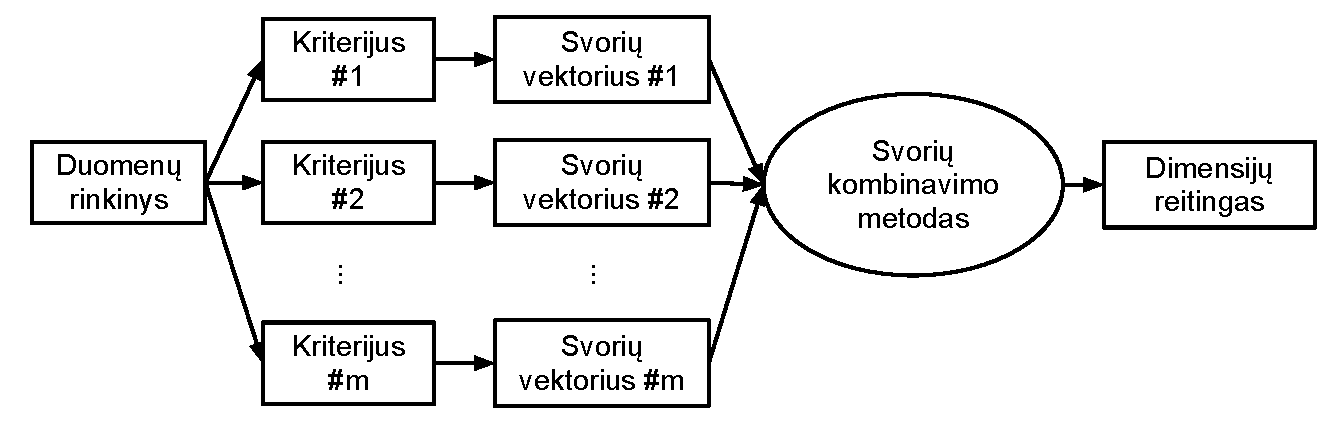
\includegraphics[width=1\textwidth]{images/score_based_fusion.pdf}
 \caption{Svoriais grįstas multikriterinis suliejimas.}
 \label{fig:figure4}
\end{figure}
\begin{figure}[ht]
\begin{minipage}[b]{0.5\linewidth}
\centering
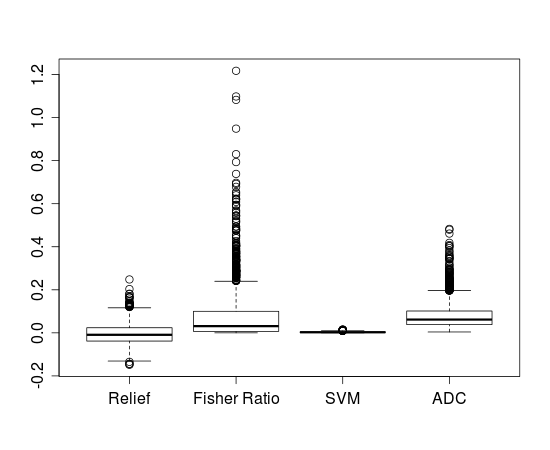
\includegraphics[width=1\textwidth]{images/boxplot_colon_all.png}
\caption{Pavienių dimensijų atrinkimo metodų nenormalizuotas svorių
pasiskirstymas.}
\label{fig:figure1}
\end{minipage}
\hspace{0.5cm}
\begin{minipage}[b]{0.5\linewidth}
\centering
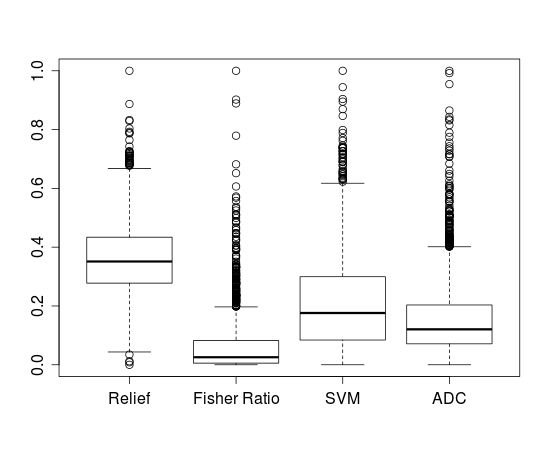
\includegraphics[width=1\textwidth]{images/boxplot_colon_all_normalized.png}
\caption{Pavienių dimensijų atrinkimo metodų normalizuotas svorių
pasiskirstymas.}
\label{fig:figure2}
\end{minipage}
\end{figure}

Suliejant svorius svarbu yra užtikrinti, kad svoriai, gauti naudojant
skirtingus bazinius kriterijus, būtų palyginami. Todėl svorių normalizavimas
turi būti atliekamas prieš svorių kombinavimą. Kitu
atveju dimensijų įvertinimo metodai bus nepalyginami. Paveikslėlyje ~\ref{fig:figure1} pav.
nenormalizuotų pavienių dimensijų vertinimo metodų skiriasi netgi suteiktų
svorių intervalai. Paveikslėlyje ~\ref{fig:figure2} pav. matome,
kad net ir normalizavus svorius gana stipriai skiriasi svorių kvartiliai - į 
tai reikia atkreipti dėmesį interpretuojant galutinius dimensijų vertinimo 
rezultatus. Šiame darbe svoriai yra 
normalizuoti intervale $[0, 1]$ pagal formulę:
\begin{equation}
 u_i'=\frac{u_i - u_{i min}}{u_{i max} - u_{i min}}, 
\end{equation}
kur $u_i$ - dimensijų svorių vektorius pagal $i$ kriterijų, 
$u_{i min}$ - minimali $u_i$ svorių vektoriaus reikšmė,
$u_{i max}$ - maksimali $u_i$ svorių vektoriaus reikšmė,
$u_i'$ - normalizuotų svorių vektorius.

Sutarties svorių vektorius $u$ yra vidurkis normalizuotų svorių vektorių:
\begin{equation}
 u = \frac{1}{m}\sum_{i=1}^m u_i',
\end{equation}
kur $m$ yra bazinių kriterijų skaičius. Reikia paminėti, kad didesnė svorio
reikšmė reiškia, kad dimensija yra geresnė.

\subsubsection{Reitingais grįstas multikriterinis suliejimas}

Reitingais grįsto multikriterinio suliejimo pagal reitingus metodas gauna
duomenų rinkinio dimensijų reitingą,
pagal keletą bazinių dimensijų reitingavimo kriterijų. Algoritmo pirmajame žingsnyje
keletas dimensijų atrinkimo kriterijų grąžina dimensijų reitingu, paskui tie
reitingai yra kombinuojami į vieną bendra dimensijų reitingą.  Algoritmas yra
pavaizduotas ~\ref{fig:figure5} pav.
\begin{figure}
 \centering
 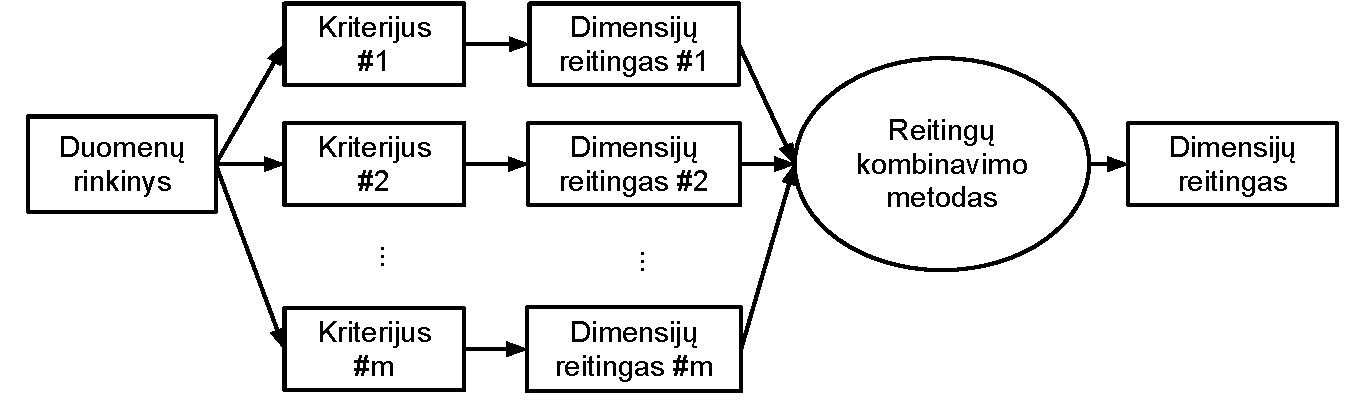
\includegraphics[width=1\textwidth]{images/ranking_based_fusion.pdf}
 \caption{Reitingais grįstas multikriterinis suliejimas.}
 \label{fig:figure5}
\end{figure}
Suliejimo pagal reitingus metodas nereikalauja dimensijų atrinkimo metodų 
rezultatų normalizavimo, nes tiesiog imame dimensijoms priskirtus reitingus ir 
juos kombinuojame. Skirtingai nei suliejimo pagal svorius algoritme, baziniai 
dimensijų atrinkimo kriterija dimensijų eliminavimas\cite{yang2011robust} susideda iš dviejų
dalių: keletos dimensijų atrinkimi turi gražinti dimensijų reitingus, o ne svorius.

Dimensijų reitingų kombinavimui yra keletas metodų\cite{dwork2001rank}, tačiau
paprastumo dėlei šiame darbe naudosiu Borda balsavimą\footnote{Dar žinomas kaip
,,Pažymių metodas``. Jis buvo pasiūlytas prancūzų matematiko ir fiziko 
Jean-Charles de Borda 1770 metais.} (angl. Borda count). Tarkime, kad turime
$m$ basuotojų ir $p$ kandidatų aibę. Tada Borda balsavimo metodas kiekvienam
$i$-ajam balsuotojui sukuria balsų vektorių $v_i$ tokiu būdu: geriausiai 
įvertintam kandidatui suteikiama $p$ taškų, antrajam kandidatui $p-1$, ir t.t.
Galutiniai taškai yra gaunami sudedant visų balsuotojų taškus
\begin{equation}
 v = \sum_{i=1}^m v_i,
\end{equation}
kur $v$ yra suminių taškų vektorius, o iš jo galime gauti ir dimensijų reitingus.

\subsubsection{Svoriais ir reitingais grįstas multikriterinis suliejimas}

Svoriais ir reitingais grįsto multikriterinio suliejimo metodas
nuo reitingais grįsto multikriterinio suliejimo metodo skiriasi tuo, kad kaip dar vienas 
reitingas yra panaudojamas svoriais grįsto multikriterinio dimensijų atrinkimo metu
gautas reitingas.
Multikriterinio dimensijų įverčių ir pagal svorius, ir pagal reitingus metodas vyksta trimis
žingsniais:
\begin{enumerate}
  \item Gauname dimensijų reitingus pagal $m$ pavienių dimensijų atrinkimo motodų;
  \item Suliejame dimensijų įverčius pagal svorius ir taip gauname vieną 
  dimensijų reitingą;
  \item Reitinguojame dimensijas pagal visus turimus $m+1$ pavienius reitingus.
\end{enumerate} 
Algoritmas yra pavaizduotas ~\ref{fig:figure3} pav.
\begin{figure}
 \centering
 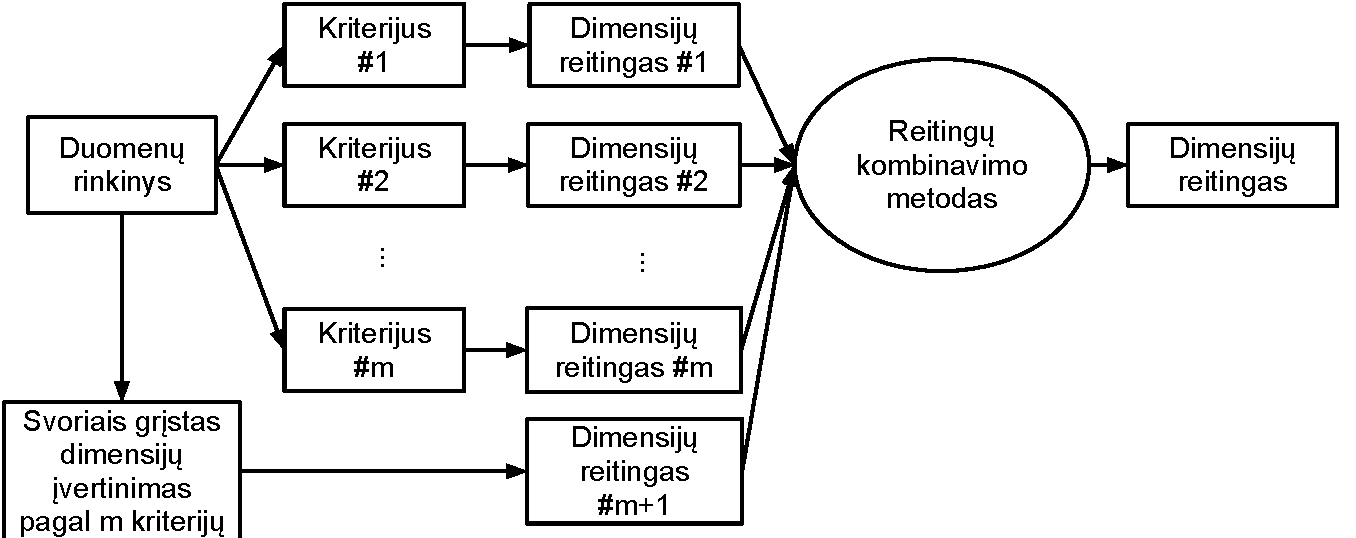
\includegraphics[width=1\textwidth]{images/score_and_ranking_based_fusion.pdf}
 \caption{Svoriais ir reitingais grįstas multikriterinis suliejimas.}
 \label{fig:figure3}
\end{figure}

Kadangi yra suliejami keli mažai koreliuojantys dimensijų reitingavimo metodai,
yra pasiekiamas didesnis dimensijų atrinkimo stabilumas, kai varijuoja 
treniravimosi duomenų poaibis (angl. subsampling).

\subsubsection{Multikriterinis rekursyvus dimensijų eliminavimas}

Jei dimensijų atrinkimo tikslas yra pagerinti klasifikavimo rezultatus, tai taikymas
multikriterinio dimensijų atrinkimo metodų nebūtinai duos pageidaujamą rezultatą,
nes yra pastebėta, kad vien dimensijų reitingavimas nebūtinai suranda geriausią dimensijų 
poaibį. Tam, kad būtų surastas geriausias dimensijų poaibis reikia kombinuoti
multikriterinį dimensijų reitingavimą su paieškos strategija. Rekursyvus 
dimensijų eliminavimas yra dažnai naudojama paieškos strategija dimensijų
atrinkimui. Todėl yra kombinuojamas multikriterinis dimensijų reitingavimas ir
rekursyvus dimensijų eliminavimas.

Multikriterinis rekursyvus dimensijų eliminavimas\cite{yang2011robust} susideda iš dviejų
dalių: keletos dimensijų atrinkimo kriterijų suliejimo ir pagal svorius, ir 
pagal reitingus, ir rekursyvaus dimensijų eliminavimo aprašyto algoritme 
nr. \ref{RFE}. Algoritmas pavaizduotas ~\ref{fig:figure6} pav.
\begin{figure}
 \centering
 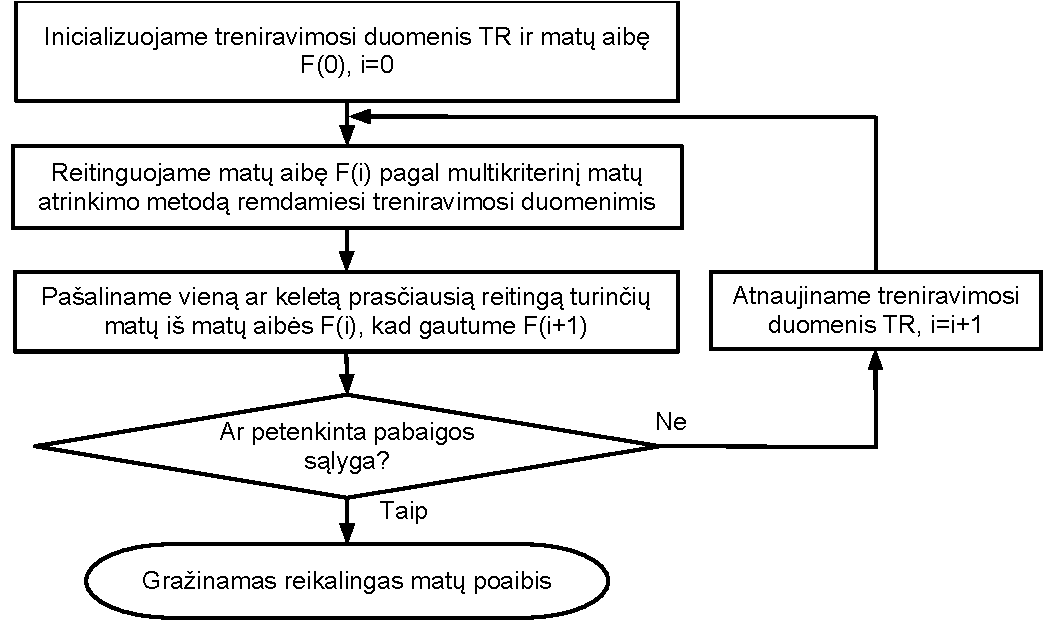
\includegraphics[width=0.7\textwidth]{images/mcf-rfe_procedure.pdf}
 \caption{Multikriterinio rekursyvaus dimensijų eliminavimo algoritmas.}
 \label{fig:figure6}
\end{figure}

Yra pastebėta, kad standartinis rekursyvus dimensijų eliminavimas, kai vienos
iteracijos metu yra eliminuojama viena dimensija, gali labai padidinti 
algoritmo sudėtingumą. Todėl genų ekspresijos duomenims yra rekomenduotina
eliminuoti keletą dimensijų vienu metu.

Nors SVM-RFE dimensijų atrinkimo algoritmas ir yra labai populiarus, tačiau yra
žinoma, kad jam trūksta stabilumo. Todėl kombinuodami didesnį stabilumą turintį
multikriterinį dimensijų atrinkimą su rekursyvaus dimensijų eliminavimo paieškos
strategija, turėtume gauti stabilesnį dimensijų atrinkimo algoritmą.

